\documentclass[12pt]{article}

\usepackage[spanish]{babel}
\usepackage[utf8]{inputenc}
\usepackage{graphicx}
\usepackage{geometry}
\usepackage{xcolor}
\usepackage{fancyhdr}
\usepackage{lastpage}
\usepackage{pdfpages}
\usepackage{listings}
\usepackage{schemata}

\geometry{top=25mm,left=15mm,right=15mm,a4paper}

\pagestyle{fancy}
\fancyhf{}
\lhead{Computación Concurrente}
\cfoot{Página \thepage\ de \pageref{LastPage}}

\graphicspath{./}

\begin{document}
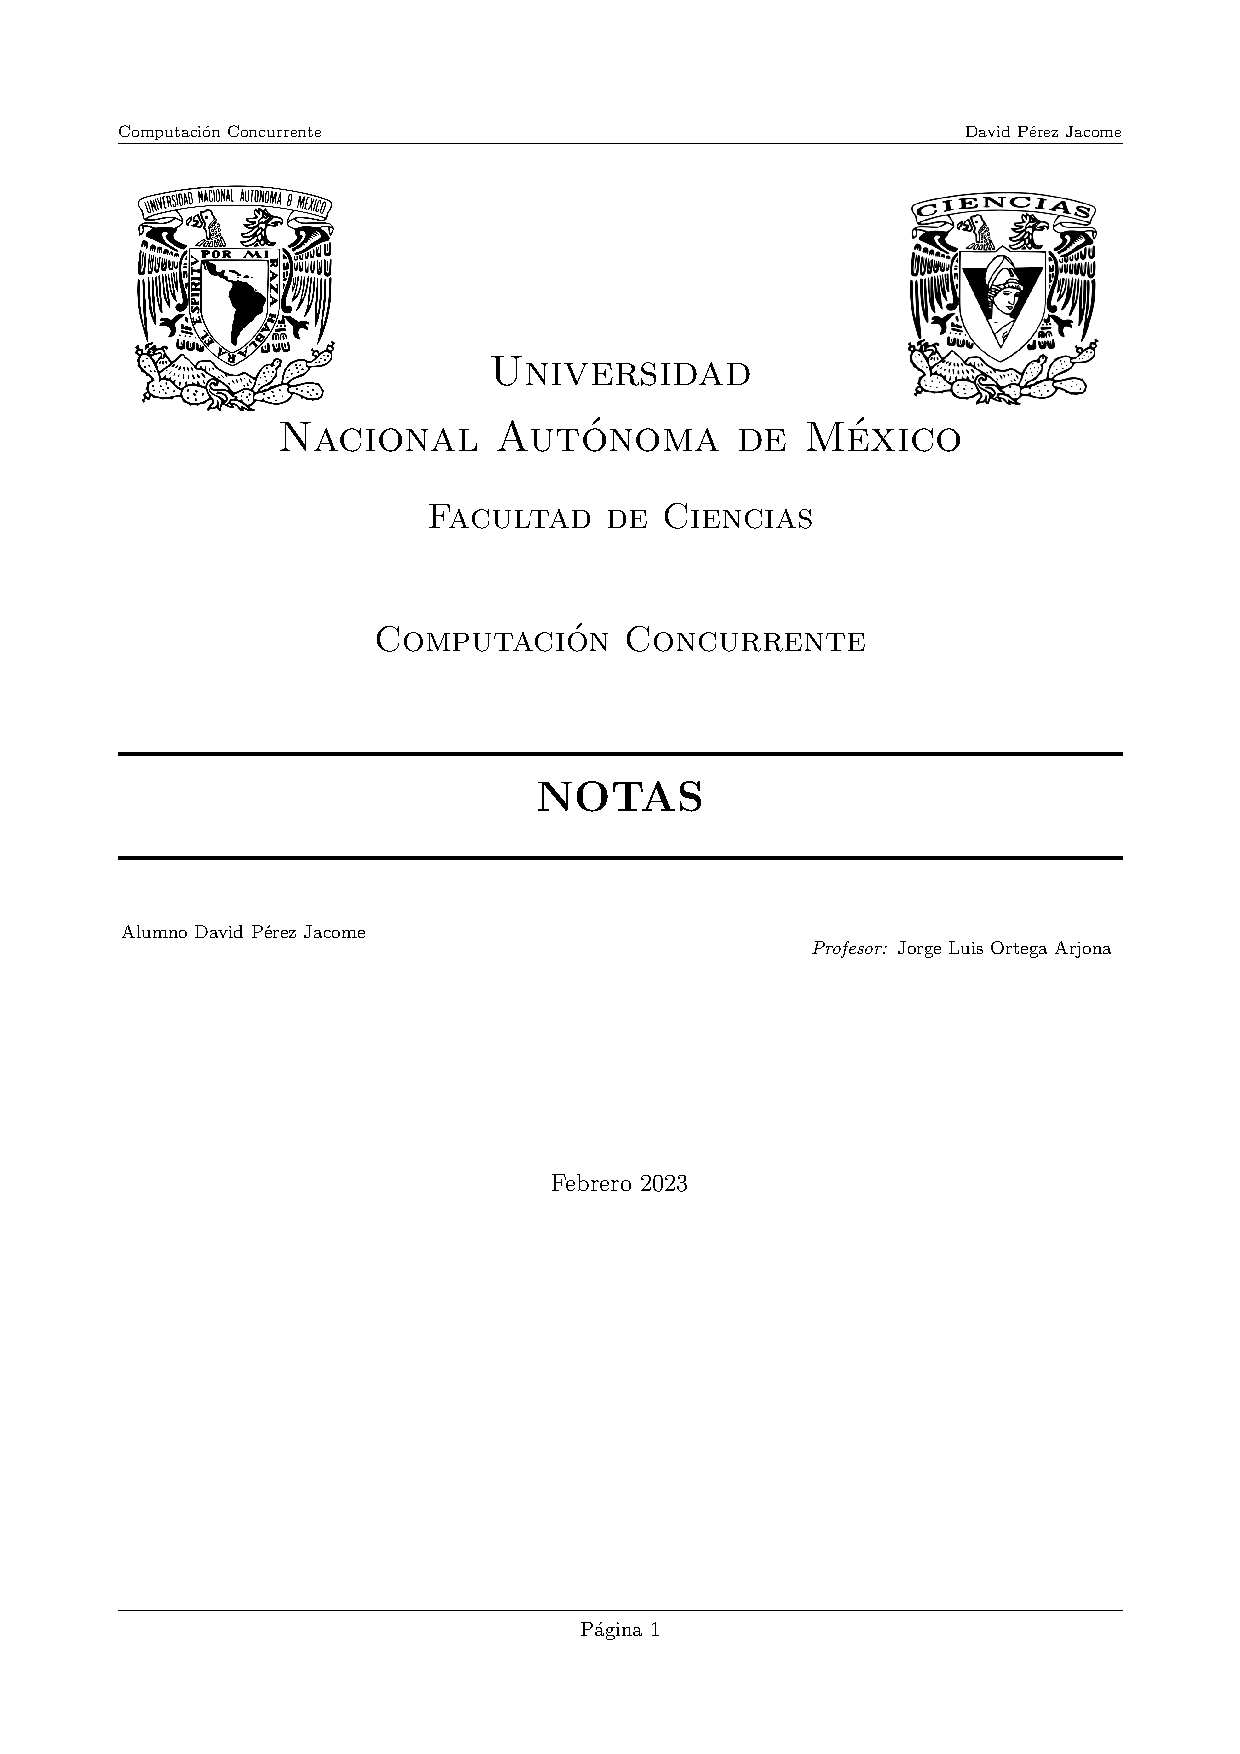
\includepdf{Portada.pdf}
{\color{blue} \section*{\textbf{Notas}}}
\vspace{1em}

{\color{blue} \subsection*{\textbf{Conceptos Fundamentales del procesamiento paralelo y distribuido.}}}

\subsubsection*{\textbf{Factores}}
\begin{enumerate}
    \item \textbf{1 Procesador}
    \begin{enumerate}
        \item tienen multithreading.
        \item memoria compartida.
    \end{enumerate}
    \item \textbf{N Procesadores} 
    \begin{enumerate}
        \item \textbf{Paralelo}(multiprocesadores o multicore).
        \begin{enumerate}
            \item \textbf{Memoria compartida}
            \begin{enumerate}
                \item Semaforos
                \item Región Critica
                \item Monitores
                \item Paso de mensajes
                \item Llamada a Proc. Remoto (RPC)
            \end{enumerate}
            \item \textbf{Memoria Distribuida}
        \end{enumerate}
        \item \textbf{Distribuido}(red de computadoras) 
    \end{enumerate}
    \item \textbf{Lenguajes de Programación}
    \item \textbf{Hardware}
\end{enumerate}
\vspace{-0.5em}
\subsubsection*{\textbf{PROGRAMACIÓN SECUENCIAL VS PROGRAMACIÓN CONCURRENTE}}
\begin{tabular}{| c | c |}
    \hline
    Secuencial & Concurrente \\ \hline
    Programa haga lo que deba hacer & Controlar el NO-Determinismo \\
    Programa que se detenga & Sincronizar procesos.
\end{tabular}
\\
\vspace{1em}

{\color{blue} \subsection*{\textbf{Factores de desempeño.}}}
\begin{enumerate}
    \item Plataforma de Hardware
    \item Lenguaje de Programación
    \item Problema de Resolución
\end{enumerate}

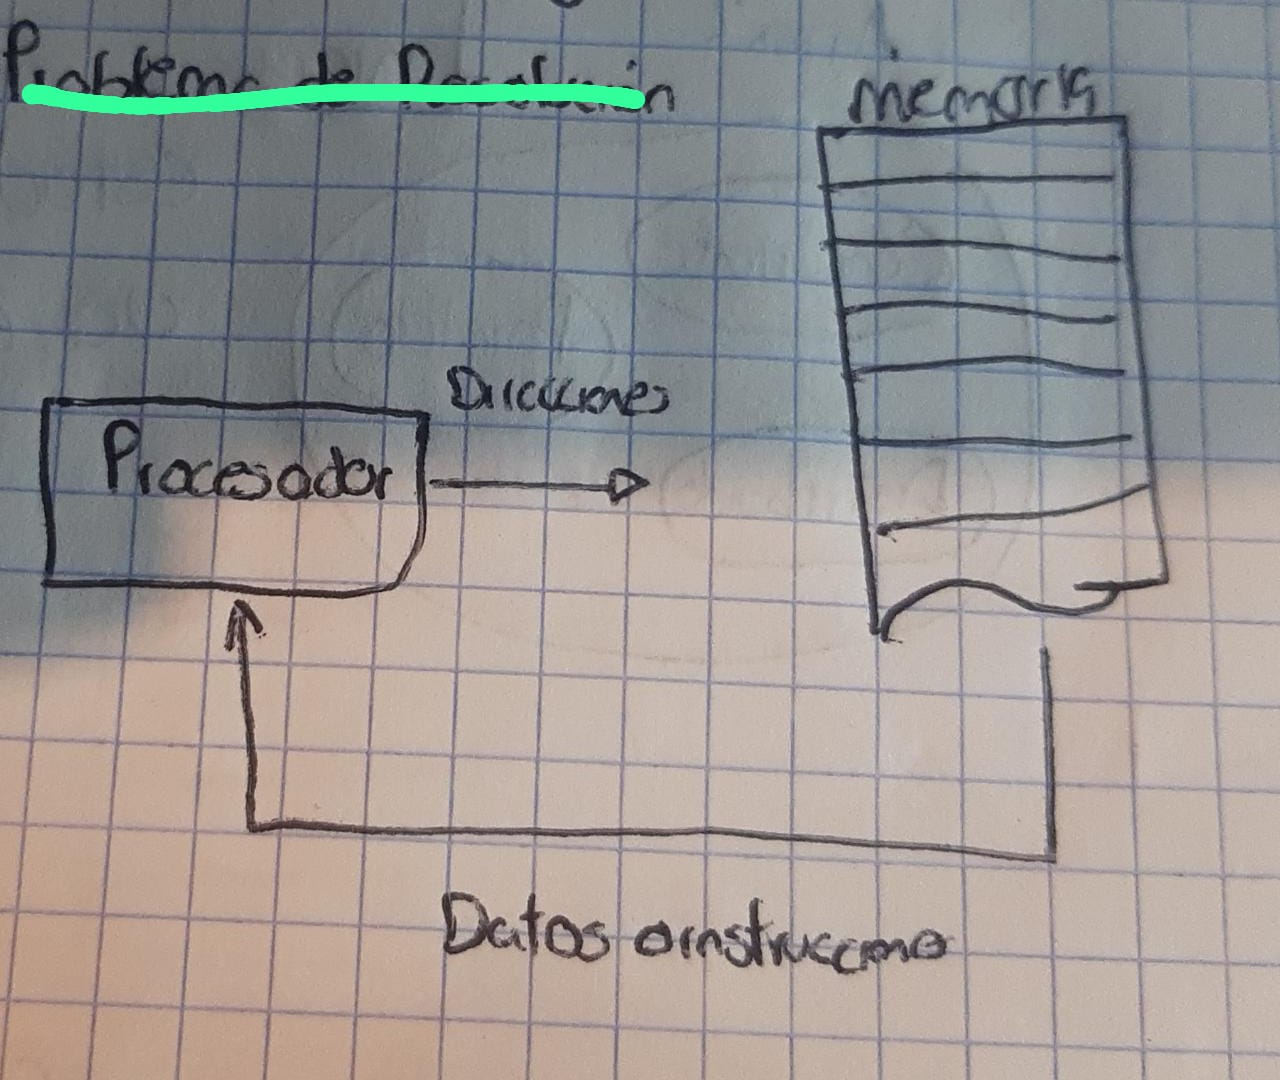
\includegraphics[scale = 0.25]{images/esquema1.jpeg} \\

{\color{blue} \subsection*{\textbf{Instrucciones y datos en memoria codificados.}}}
En la ejecución de un programa se siguen varios pasos, como lo son:\\
\begin{enumerate}
    \item FETCH: Obtener o buscar las instruciones.
    \item DECODE: De que trata (decodificación).
    \item EXECUTE: Ejecución de la instrucción.
    \item WRITE: Se escribe en el caso de sincronia para el proceso.
\end{enumerate}

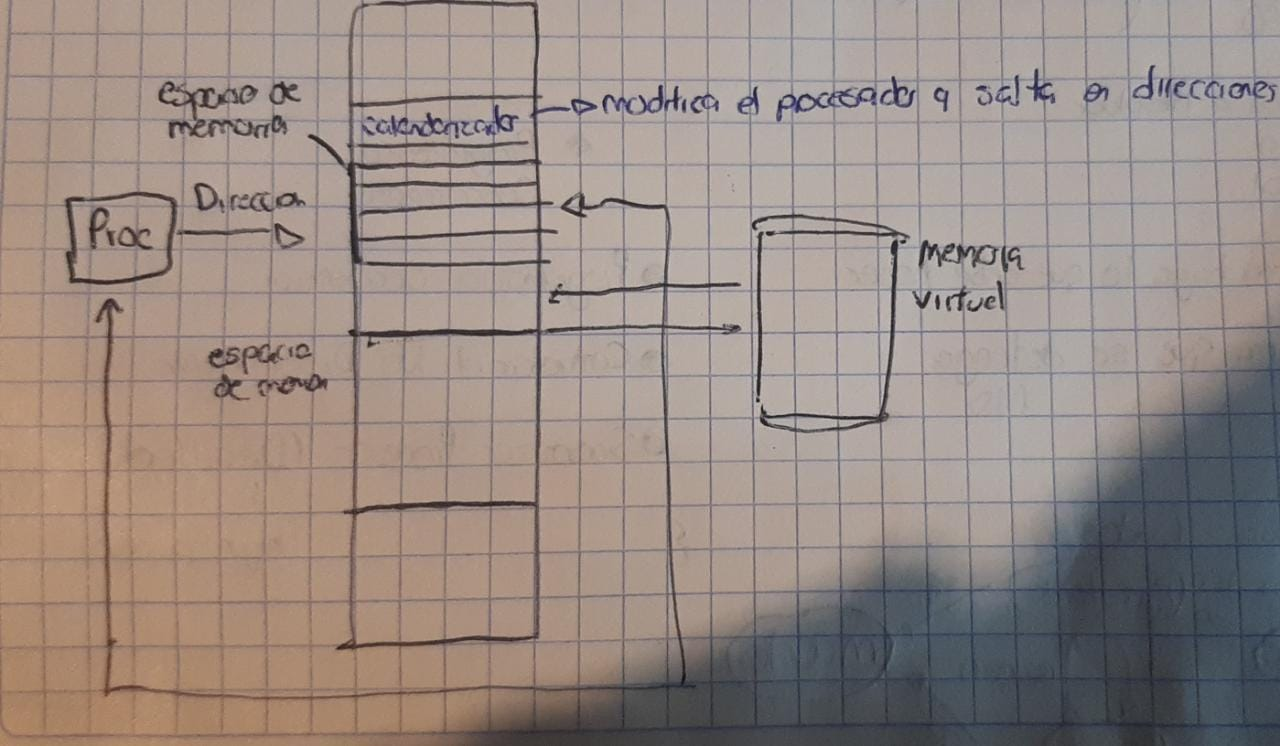
\includegraphics[scale = 0.30]{images/esquema2.jpeg} \\

{\color{blue} \subsection*{\textbf{Memoria compartida.}}}
Se encarga de comunicar procesos mediante la variable global (\textbf{Variable Compartida}).
Todos los procesadores acceden a una memoria global \\

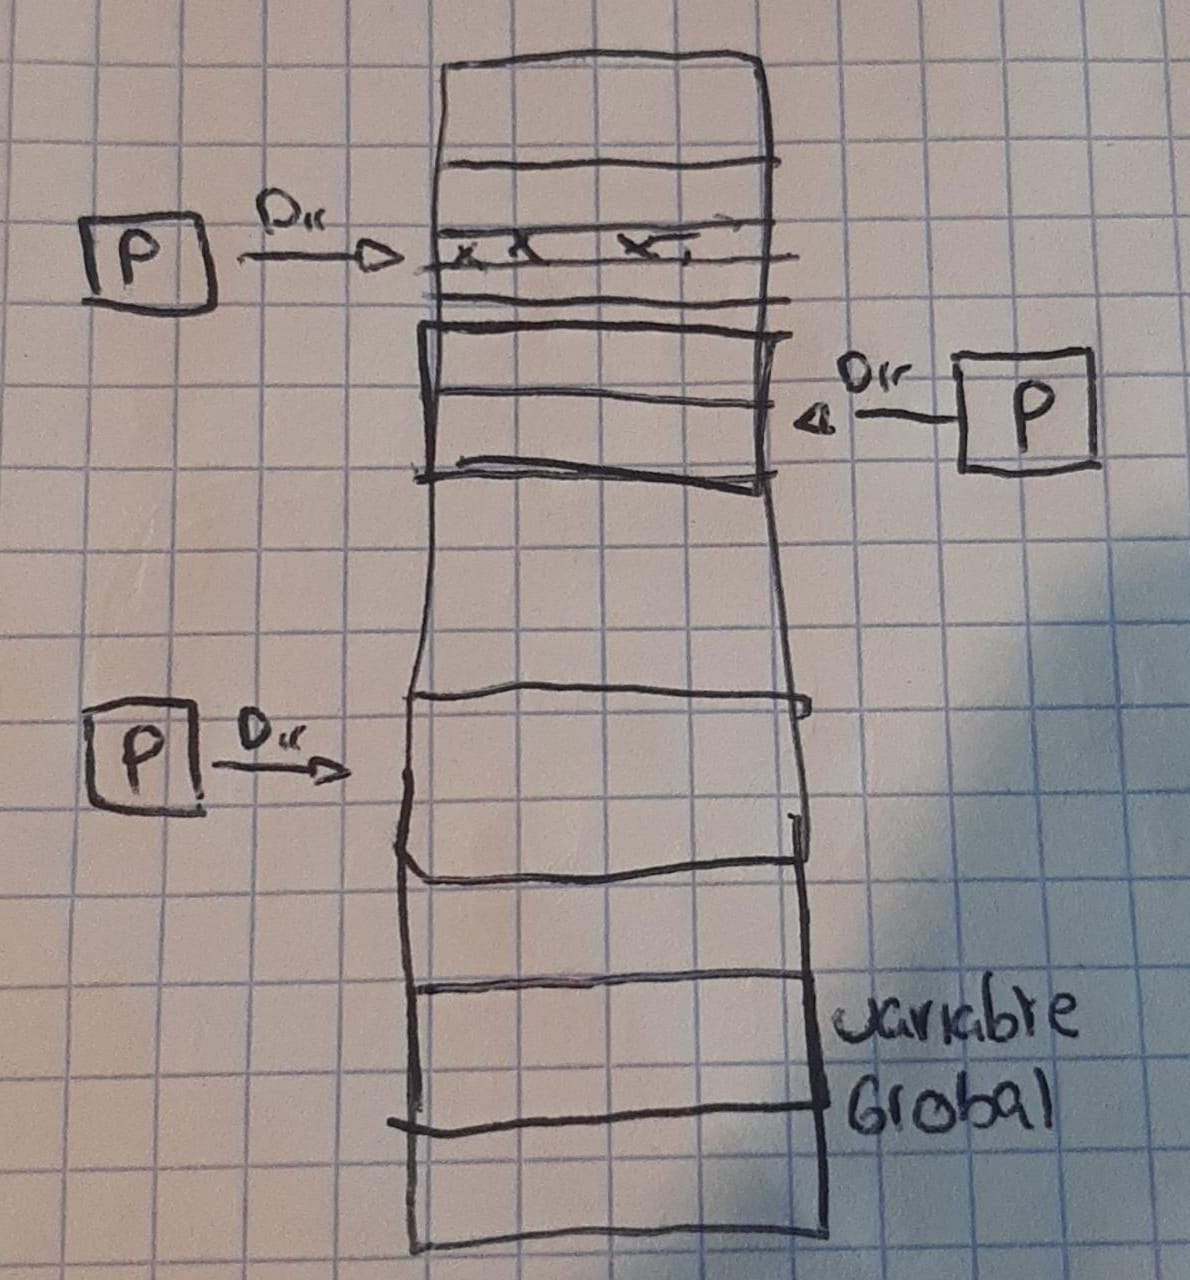
\includegraphics[scale = 0.30]{images/esquema3.jpeg} \\

{\color{blue} \subsection*{\textbf{Memoria Distribuida.}}}
Cada procesador tiene su memoria local intercambiando datos mediante una red de comunicación \textbf{(E/S)}\\

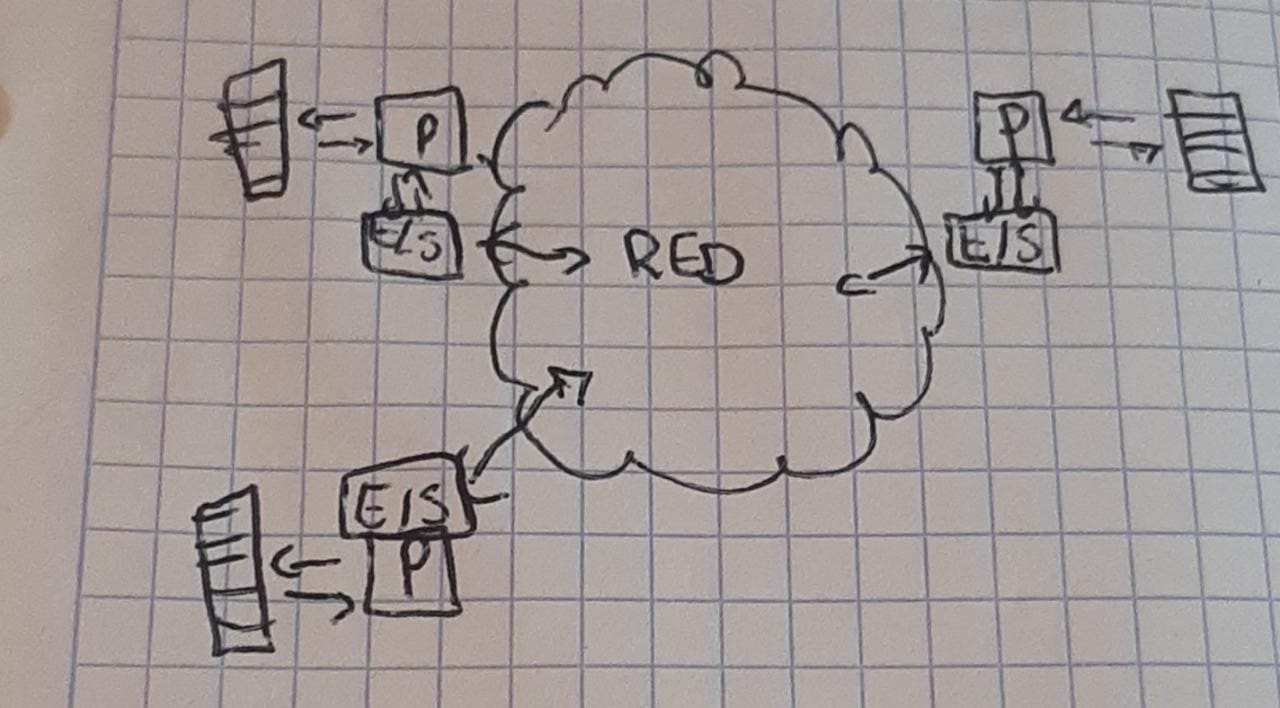
\includegraphics[scale = 0.35]{images/esquema4.jpeg} \\

{\color{blue} \subsection*{\textbf{LENGUAJE DE PROGRAMACIÓN.}}}
\vspace{1em}

\begin{enumerate}
    \item \textbf{Expresar Concurrencia:} OCAN: PAR, ---- parbegin y parend. {\color{red}*preguntar el leguaje occan y otro}
    \item \textbf{Expresar Secuencialidad:} ($P_{1}; P_{2}$;) instrución secuencial, OCCAN: (SEQ)
    \item \textbf{Expresar Comunicación:} Depende de la organización de la memoria.
    \begin{enumerate}
        \item \textbf{Compartida:} Variable Compartida.
        \item \textbf{Distribuida:} Llamada a procedimientos Remotos y paso de mensajes \color{red} send(), recerver()
    \end{enumerate}
    \item \textbf{Control del NO-Determinismo:} No todos, esto significa que antes de ejecutarlo no sabremos que pasará. Conjunto de 
    estados no se sigue rigurosamente.\\
    Instrución alternativa de Dijktra: Instrucción concurrentemente o al mismo tiempo y sin parar.
\end{enumerate}

(threads en java nos dan la concurrencia)

{\color{blue} \subsection*{\textbf{Inclusión de concurrencia en Lenguajes de Programación.}}}
\begin{enumerate}
    \item Diseño del Lenguaje (Occan).
    \item Modificando el lenguaje.(extención en el compilador).
    \item Utilizando bibliotecas (libres).
\end{enumerate}
\vspace{2em}

{\color{blue} \subsubsection*{\textbf{Problema a Resolver.}}}

Programa $=$ Algoritmo $+$ Datos.

({\color{red} \textbf{Capacidad de dividir el algoritmo ó datos para programar en paralelo.}})\\

{\color{red} \textbf{Programa Concurrente:}} Componentes de procesamiento $+$ Componentes de comunicación.\\

{\color{blue} \subsection*{\textbf{Conceptos y Terminología.}}}
\vspace{1em}

{\color{red} \textbf{Proceso.}} Es el cambio en el \textbf{estado} de la memoria por acción del procesador. (valor instantaneo de las variables de un sistema.)\\

{\color{red} \textbf{Programa.}} Es la especificación de uno o varios procesos. (ya sea \textbf{secuencial} o \textbf{concurrente}.)
\vspace{2em}\\

\begin{enumerate} 
    \item {\color{red} \textbf{Programación Secuencial.}} Especificación de un proceso.
    \item {\color{red} \textbf{Programación Concurrente.}} Especificación de varios procesos.\\
    Conjunto de de procesos secuenciales que se ejecutan simultaneamente, comunican entre si por un objetivo en común.
    \begin{enumerate}
        \item \textbf{Programa Multithread.}
        \item \textbf{Programa Paralelo.}
        \begin{enumerate}
            \item Memoria compartida: comunicación por memoria.
            \item Memoria Distribuida: Reedes Compartidas.
        \end{enumerate}
        \item \textbf{Programas Distribuidos.}
    \end{enumerate}
\end{enumerate}

\begin{tabular}{| c | c |}
    \hline
    \textbf{Cnceptos de SW} & \textbf{Cnceptos de HW} \\ \hline
    Proceso & Procesador \\
    Comunicación(variable compartida (global.\\
    Paso de mensajes y llamadas a procedimientos remotos)) & Memoria (Distrib y Compartida).
\end{tabular}\\

*(procesador accede a la memoria en nano segundos)\\
* Los factores son: plataforma de HW, lenguajes de programación y el problema a resolver.
\vspace{2em}

{\color{blue} \subsubsection*{\textbf{Coordinación.}}}
\vspace{1em}

{\color{blue} \subsubsection*{\textbf{Comunicación.}}}
\vspace{1em}

{\color{blue} \subsubsection*{\textbf{Sincronización.}}}
\vspace{1em}

{\color{blue} \subsubsection*{\textbf{Granularidad..}}}
\vspace{1em}









\end{document}